\documentclass[sigconf,nonacm]{acmart}

\settopmatter{printacmref=false}
\renewcommand\footnotetextcopyrightpermission[1]{}
\pagestyle{plain}

\usepackage{kotex}
\usepackage{booktabs}
\usepackage{array}
\usepackage{graphicx}

\title{Beyond Aggregate Metrics: Attack-Type-Specific Evaluation of Flow-Level IDS Models}

\author{Yonghyeon Lee}
\email{yhylee@ucdavis.edu}
\affiliation{%
  \country{}
}

\begin{abstract}
Network intrusion detection 연구는 종종 precision, recall, F1-score 같은 aggregate metric으로 모델을 비교한다.
이 metric들은 high-level model comparison에는 유용하지만, 서로 다른 attack behavior를 하나의 score로 압축하면서 어떤 attack type이 uncovered로 남는지 숨길 수 있다.
특히 쉬운 high-signal attack에서 높은 성능을 내면 모델이 overall로 reliable해 보일 수 있지만, rare하거나 stealthy하거나 운영상 중요한 attack category의 false negative는 평균 속에 묻힐 수 있다.
이 논문은 neural model과 traditional machine learning model의 비교를 experimental lens로 사용해, flow-level intrusion detection에서 이러한 한계를 분석한다.
CSE-CIC-IDS2018 processed flow-feature dataset을 사용해 Logistic Regression, Random Forest, Shallow MLP, Lightweight PyTorch MLP, Deep MLP, Autoencoder + MLP를 같은 binary benign/malicious task로 학습했고, post-hoc attack-type analysis를 위해 원래 attack label을 보존했다.
결과는 aggregate metric과 attack-type-specific false negative가 서로 다른 model choice를 지지할 수 있음을 보여준다.
Deep MLP와 Autoencoder + MLP는 precision과 F1-score를 개선했지만, Logistic Regression이 가장 높은 attack recall과 가장 낮은 false-negative rate를 보였다.
Attack-type analysis는 DoS/DDoS와 많은 brute-force attack이 잘 탐지되고, Random Forest가 Bot과 SQL Injection에서 가장 강하며, Infiltration은 모든 모델의 shared blind spot으로 남는다는 점을 보여준다.
이 결과는 attack-type-specific analysis가 단순한 해석 보조가 아니라 모델 선택, threshold 조정, 그리고 각 모델이 잘 cover하는 attack family를 중심으로 더 유연한 hybrid IDS를 설계하기 위한 핵심 평가 단계임을 시사한다.
다시 말해 aggregate metric은 평균적으로 좋은 모델을 보여주지만, attack-type analysis는 그 모델이 특정 IDS 환경에서 중요한 attack family를 실제로 cover하는지 보여준다.
따라서 IDS evaluation은 하나의 global winner를 고르는 방식에서 벗어나, aggregate metric과 attack-type-specific false-negative analysis를 함께 사용해 미래 IDS 설계가 더 다양한 coverage-oriented 선택지를 가질 수 있게 해야 한다.
\end{abstract}

\keywords{intrusion detection, neural networks, Random Forest, false negatives, CSE-CIC-IDS2018, attack-type evaluation}

\begin{document}
\maketitle

\section{Introduction}

Network intrusion detection system은 network activity를 benign 또는 suspicious로 분류해 방어자가 malicious traffic을 조사하거나 차단할 수 있게 한다.
많은 machine learning 기반 IDS 연구에서는 accuracy나 F1-score 같은 aggregate score가 headline result로 제시된다.
이런 방식은 모델을 전체적으로 비교하는 데에는 유용하지만, security analysis에는 충분하지 않다.
운영 환경의 IDS에서는 오류의 비용이 서로 다르다.
False positive는 analyst workload를 증가시키지만, false negative는 malicious traffic이 탐지되지 않고 통과했다는 뜻이다.
따라서 어떤 모델이 높은 aggregate score를 보여도 특정 attack family를 반복적으로 놓친다면 보안적으로 위험할 수 있다.

본 연구는 이 문제를 flow-level intrusion detection setting에서 분석한다.
Flow-level data는 packet 하나하나의 내용을 직접 다루기보다, 여러 packet으로 이루어진 하나의 network flow를 요약한 feature로 표현한다.
예를 들어 packet count, byte count, flow duration, rate, inter-arrival timing, TCP flag behavior 같은 값이 사용된다.
이 방식은 raw packet trace를 그대로 분석하는 것보다 가볍고 재현하기 쉬워서, 여러 모델을 같은 조건에서 비교하는 quarter-scale study에 적합하다.
또한 이런 tabular feature는 traditional machine learning model과 neural network model 모두에 사용할 수 있다.
하지만 이 장점이 곧 한계도 만든다.
모델을 binary benign/malicious task로만 평가하면, 전체적으로 공격을 얼마나 잘 잡았는지는 볼 수 있지만 어떤 attack type을 놓쳤는지는 잘 보이지 않을 수 있다.
따라서 본 연구의 핵심 문제는 높은 aggregate IDS score가 실제로는 특정 attack type의 낮은 coverage를 가리고 있는지 확인하는 것이다.

이 문제의식은 다음 research question으로 이어진다.
\emph{Flow-level IDS model을 평가할 때 aggregate metric은 어떤 한계를 가지며, 그 한계는 어떻게 보완될 수 있는가?}
이 질문의 목적은 단순히 best IDS model을 고르는 것이 아니다.
핵심은 높은 aggregate score를 가진 모델도 중요한 attack type을 놓칠 수 있는지 확인하는 것이다.
이를 위해 본 연구는 neural model과 traditional model을 같은 pipeline에서 비교한다.
그리고 DoS/DDoS, brute force, botnet, infiltration, web-based attack별로 각 모델이 어디서 잘 작동하고 어디서 실패하는지 살펴본다.
이 attack-type result는 모델 선택, 오류 원인 분석, future hybrid IDS design을 위한 근거로도 사용될 수 있다.
이 관점에서 attack-type-specific evaluation은 단순한 post-hoc explanation이 아니라 practical model selection으로 확장된다.
Aggregate metric은 평균적으로 좋은 모델을 보여주지만, attack-type analysis는 그 모델이 특정 IDS 환경에서 중요한 attack family를 실제로 cover하는지 보여준다.

초기 hypothesis는 aggregate metric만으로는 각 모델의 security coverage를 충분히 설명하지 못한다는 것이었다.
나는 neural model이 일부 aggregate score를 개선하고, botnet이나 web-based traffic처럼 feature interaction이 중요한 attack에서 더 나은 성능을 보일 수 있다고 예상했다.
반대로 high-volume DDoS traffic처럼 feature pattern이 비교적 뚜렷한 공격에서는 Random Forest 같은 traditional model도 여전히 강할 것으로 예상했다.
따라서 더 넓은 hypothesis는 모델 종류마다 남기는 blind spot이 다르며, attack-type-specific false-negative analysis가 aggregate metric 속에 숨겨진 security-relevant difference를 드러낼 것이라는 점이다.

이 연구의 theoretical contribution은 aggregate IDS metric이 security-relevant false negative를 어떻게 숨길 수 있는지 보여주는 attack-type-specific evaluation framework이다.
이 framework는 모델 성능을 하나의 aggregate score로 요약하는 대신, 각 모델이 어떤 attack type을 탐지하고 어떤 attack type을 uncovered로 남기는지 비교한다.
따라서 model comparison은 단순한 ranking이 아니라, 각 model family가 어떤 traffic pattern에 강하거나 약한지를 드러내는 diagnostic procedure로 해석된다.
Empirical contribution은 같은 CSE-CIC-IDS2018 sample에서 Logistic Regression, Random Forest, Shallow MLP, Lightweight PyTorch MLP, Deep MLP, Autoencoder + MLP를 같은 pipeline으로 학습하고, model-level 및 attack-level false negative를 함께 보고하는 reproducible implementation이다.
최종 결과는 neural model이 일부 aggregate metric을 개선할 수는 있지만, missed attack을 일관되게 줄이지는 못하며, 특히 Infiltration 같은 attack type의 blind spot은 aggregate score만으로는 드러나지 않는다는 점을 보여준다.

\section{Related Work}

이 프로젝트는 IDS model performance를 해석하는 방식의 gap에서 출발한다.
Gamage and Samarabandu는 IDS model comparison이 서로 다른 dataset과 evaluation metric 때문에 어렵다고 설명하며, benchmark에서 accuracy, F1-score, false-positive rate, false-negative rate 같은 model-level metric을 보고했다 [1].
하지만 dataset이 imbalanced하거나 일부 attack category가 더 어려운 경우 aggregate score는 security-relevant failure를 숨길 수 있다.
Saito and Rehmsmeier는 imbalanced classification problem에서 precision-recall analysis가 특히 informative하다는 점을 보였다 [2].
IDS에서는 false negative가 system이 놓친 malicious flow를 의미하므로, 본 연구는 recall, false-negative rate, attack-type detection rate를 핵심 security metric으로 다룬다.

CSE-CIC-IDS2018은 본 연구의 empirical setting을 제공한다.
이 dataset은 brute force, Heartbleed, botnet, DoS, DDoS, web attack, infiltration을 포함하는 여러 attack scenario를 제공한다 [3].
본 연구에서는 이 dataset을 binary benign/malicious task로 학습하면서도 원래 attack label을 보존해 post-hoc attack-category analysis를 수행할 수 있다는 점이 중요하다.

IDS modeling prior work는 본 연구의 model set을 정당화한다.
Logistic Regression은 linear baseline으로 사용하고, Random Forest는 many decision-tree predictor를 ensemble로 결합하는 standard traditional machine learning baseline으로 사용한다 [4].
Deep learning도 IDS에서 활발히 연구되었다: Gamage and Samarabandu는 feed-forward neural network, autoencoder, deep belief network, LSTM을 비교했고 [1], Rosay, Carlier, Leroux는 CICIDS2017에서 MLP 기반 IDS가 경쟁력 있음을 보였으며 [5], Song, Hyun, Cheong은 autoencoder의 capacity, latent size, thresholding이 IDS performance에 큰 영향을 줄 수 있음을 보였다 [6].
이 prior work는 traditional model, MLP 기반 model, autoencoder 기반 model을 함께 비교할 이유를 제공하지만, neural architecture를 추가하는 것만으로는 충분한 contribution이 아니라는 점도 보여준다.
따라서 본 논문은 이 baseline들을 사용해 common model-comparison metric이 threat landscape 전반의 attack-specific false-negative pattern을 가리는지 묻는다.

\section{Method}

\subsection{Dataset and Filtering}

이 연구는 CSE-CIC-IDS2018 processed traffic data for machine learning을 사용한다.
Raw file은 public AWS S3 bucket에서 다운로드했고, reproducible sampled dataset으로 처리했다.
최종 sample은 50,000개 flow, 79개 numeric flow feature, 37,308개 benign flow, 12,692개 attack flow를 포함한다.
전처리 과정에서는 binary model output을 이후 attack type별로 분석할 수 있도록 14개 fine-grained attack label을 보존했다.

모델 학습 task는 binary classification이다.
각 row는 benign 또는 malicious로 labeling된다.
Original attack label은 prediction target으로 사용하지 않는다.
연구 질문이 aggregate binary IDS metric이 attack type별 failure를 숨기는지에 있기 때문이다.
대신 original label은 train, validation, test split 전체에서 보존되고 post-hoc evaluation에만 사용된다.

Preprocessing pipeline은 column name cleaning, label column detection, non-feature metadata column removal, missing/infinite value replacement, numeric feature scaling, train/validation/test split을 수행한다.
최종 split은 training 32,000 rows, validation 8,000 rows, test 10,000 rows이다.
Random seed는 reproducibility를 위해 42로 고정했다.
Sampling 과정에서는 rare attack category가 제거되지 않도록 rare-label preservation을 사용했다.

\subsection{System Building Blocks}

구현된 system은 lightweight flow-level IDS prototype이다.
네 개의 주요 building block으로 구성된다.
첫째, dataset preparation script는 raw CSE-CIC-IDS2018 CSV file을 읽고 attack label을 보존하는 sampling을 수행한 뒤 processed training CSV를 생성한다.
둘째, training pipeline은 processed CSV를 로드하고 shared preprocessing pipeline을 적용한 뒤, 선택된 모든 모델을 학습하고 artifact를 저장한다.
셋째, evaluation module은 binary metric, attack-type detection summary, attack-family detection summary, plot을 생성한다.
넷째, prediction module은 saved artifact를 로드해 새로운 CSV file에 trained model을 적용한다.

System은 Python, pandas, NumPy, scikit-learn, PyTorch, matplotlib로 구현되었다.
scikit-learn은 Logistic Regression, Random Forest, scaling, splitting, metric computation에 사용되었다.
PyTorch는 neural model과 training loop에 사용되었다.
Repository에는 data preparation, training, prediction을 재현하기 위한 README command도 포함되어 있다.

\subsection{Models}

총 여섯 개 모델을 비교했다.
여섯 모델은 complexity와 inductive bias가 서로 다르기 때문에, 서로 다른 aggregate score가 서로 다른 attack-type blind spot과 연결되는지 확인할 수 있다.
Logistic Regression은 simple linear baseline이며 balanced class weight를 사용한다.
Random Forest는 traditional non-neural baseline이며 balanced subsampling을 사용한다.
Neural baseline은 Shallow MLP, Lightweight PyTorch MLP, Deep MLP, Autoencoder + MLP이다.
Shallow MLP는 하나의 hidden layer를 가진다.
Lightweight PyTorch MLP는 기존 two-hidden-layer model이다.
Deep MLP는 feed-forward layer를 더 많이 사용해 depth 증가가 attack recall을 개선하는지 확인한다.
Autoencoder + MLP는 먼저 compressed latent representation을 학습한 뒤 그 representation을 classifier에 입력한다.

모든 모델은 같은 split에서 학습 및 평가되었다.
이를 통해 비교의 초점을 data difference가 아니라 model behavior에 맞췄다.
Neural model은 leaderboard-style optimization이 아니라 attack-specific failure pattern 비교를 위한 reproducible baseline으로 구현했기 때문에 과도한 tuning은 하지 않았다.

\subsection{Measures}

주요 metric은 precision, recall, F1-score, false-negative rate, attack-type detection rate, attack-family detection rate이다.
Binary malicious class에서 recall은 전체 attack 중 탐지된 비율을 의미한다.
False-negative rate는 1 minus recall이며, 놓친 attack의 비율을 직접 측정한다.
Precision은 malicious로 예측한 flow 중 실제 malicious flow의 비율이다.
F1-score는 precision과 recall을 균형 있게 반영한다.
TP, FP, FN은 각각 malicious class에 대한 true positive, false positive, false negative를 의미한다.
Aggregate metric은 다음과 같이 계산했다.
\begin{equation}
\begin{aligned}
\mathrm{Precision} &= \frac{TP}{TP + FP}, \\
\mathrm{Recall} &= \frac{TP}{TP + FN}, \\
\mathrm{F1} &= \frac{2 \cdot \mathrm{Precision} \cdot \mathrm{Recall}}
{\mathrm{Precision} + \mathrm{Recall}}, \\
\mathrm{FNR} &= \frac{FN}{TP + FN} = 1 - \mathrm{Recall}.
\end{aligned}
\end{equation}

Recall과 attack-type detection rate의 차이는 계산 범위에 있다.
Recall은 전체 malicious test flow를 대상으로 계산하는 aggregate metric이다.
반면 attack-type detection rate는 특정 attack type 또는 attack family 안에서만 계산하는 group-specific recall이다.
즉 새로운 종류의 metric이라기보다, recall을 attack label별로 나누어 본 값이다.

\begin{table}[t]
  \caption{Overall recall과 attack-type detection rate의 차이.}
  \label{tab:recall_definition}
  \centering
  \small
  \begin{tabular}{@{}p{0.22\linewidth}p{0.30\linewidth}p{0.32\linewidth}@{}}
    \toprule
    Metric & 계산 범위 & 해석 \\
    \midrule
    Overall recall & 전체 malicious test flow & 전체 attack 중 모델이 탐지한 비율 \\
    Attack-type detection rate & 특정 attack type 또는 family의 malicious flow & 해당 attack group 안에서 모델이 탐지한 비율 \\
    \bottomrule
  \end{tabular}
\end{table}

Attack-type detection rate, 또는 attack-type recall은 malicious test row를 original fine-grained attack label별로 grouping한 뒤, 각 모델이 malicious로 탐지한 row의 비율을 계산한다.
Attack-family detection rate, 또는 attack-family recall은 fine-grained label을 Botnet, Brute Force, DoS/DDoS, Infiltration, Web Attack의 다섯 broad group으로 mapping한 뒤 같은 방식으로 계산한다.
이 두 수준의 분석이 모두 필요하다.
Fine-grained view는 구체적인 failure case를 보여주고, family-level view는 broader security pattern을 요약한다.
이 group-level metric은 aggregate precision, recall, F1-score를 보완해 어떤 attack category가 uncovered로 남는지 보여준다.
Attack type 또는 family \(g\)에 대한 group-specific recall은 다음과 같이 계산했다.
\begin{equation}
\mathrm{DetectionRate}(g) =
\frac{\sum_{i \in G_g} \mathbf{1}[\hat{y}_i = 1]}
{|G_g|},
\end{equation}
여기서 \(G_g\)는 original label이 group \(g\)에 속하는 malicious test flow의 집합이고, \(\hat{y}_i=1\)은 model이 flow \(i\)를 malicious로 예측했다는 의미이다.
예를 들어 Random Forest는 Botnet family의 24개 test flow 중 23개를 malicious로 탐지했다.
따라서 Botnet에 대한 detection rate는 다음과 같다.
\[
\mathrm{DetectionRate}(\mathrm{Botnet}) = 23/24 = 0.958.
\]
반대로 Logistic Regression은 Infiltration family의 1,669개 test flow 중 499개만 탐지했다.
따라서 Infiltration에 대한 detection rate는 다음과 같다.
\[
\mathrm{DetectionRate}(\mathrm{Infiltration}) = 499/1669 = 0.299.
\]
이처럼 같은 수식은 어떤 attack group이 거의 covered되었는지, 또는 여전히 major blind spot으로 남았는지를 직접 보여준다.

\subsection{Implementation and Reproducibility}

실험은 manually edited notebook이 아니라 reproducible command-line pipeline으로 실행되었다.
여러 모델과 여러 attack category를 비교하는 연구에서는 작은 manual step도 결과 해석을 흔들 수 있다.
예를 들어 어떤 모델만 다른 train/test split에서 평가되거나, 어떤 결과만 다른 preprocessing을 거치면 model comparison 자체가 불공정해진다.
따라서 본 연구의 implementation은 데이터 준비, 학습, 평가가 같은 순서와 같은 설정으로 반복되도록 구성했다.

Pipeline은 먼저 CSE-CIC-IDS2018 flow-level data를 정리하고, rare attack label이 사라지지 않도록 sampling을 적용한다.
그 다음 모든 모델에 동일한 train/validation/test split을 사용한다.
이렇게 하면 Logistic Regression, Random Forest, MLP 계열 모델, Autoencoder + MLP가 같은 test traffic에 대해 비교된다.
또한 binary benign/malicious label은 training target으로 사용하지만, original attack label은 evaluation 단계까지 보존한다.
이 설계 덕분에 overall precision, recall, F1-score뿐 아니라 attack-type별 detection rate와 false negative도 같은 기준에서 계산할 수 있다.

최종 실행에서는 여섯 개 모델을 모두 같은 pipeline에서 학습하고 평가했다.
실험 결과는 aggregate metric, false-negative comparison, attack-type result, attack-family result로 정리되었다.
중요한 점은 특정 모델의 결과를 개별적으로 손으로 조정한 것이 아니라, 같은 evaluation procedure가 모든 모델에 적용되었다는 것이다.
또한 학습된 모델을 다시 불러와 새로운 CSV traffic에 prediction을 수행할 수 있도록 prediction step도 포함했다.
따라서 이 프로젝트는 단순한 result table 작성이 아니라, 동일한 데이터 처리와 평가 절차를 반복할 수 있는 작은 IDS evaluation system으로 구현되었다.
재현성을 위해 source code와 생성된 experiment output은 \url{https://github.com/section9-us/Network_ids-neural-vs-traditional-attack-eval}에 공개되어 있다.

\section{Results}

\subsection{Overall Model Performance}

10,000-row test split의 binary malicious-class performance는 본 연구의 central tension을 보여준다.
Aggregate F1-score는 Deep MLP를 지지하지만, security-focused false-negative metric은 Logistic Regression을 지지한다.
Deep MLP는 가장 높은 precision과 F1-score(precision 0.747, F1 0.574)를 보인 반면, Logistic Regression은 가장 높은 recall과 가장 낮은 false-negative rate(recall 0.528, FNR 0.472)를 보였다.
이 차이는 실험의 security interpretation에서 핵심적이다.
F1-score 기준으로 가장 좋아 보이는 모델이 공격을 가장 적게 놓치는 모델은 아니었다.
모델별로 보면 Logistic Regression은 가장 적은 attack을 놓쳤고(1,197개), Shallow MLP는 neural model 중 가장 높은 recall을 보였다(recall 0.524, missed attack 1,209개).
PyTorch MLP는 중간 정도의 precision-recall tradeoff를 보였지만, Deep MLP와 Autoencoder + MLP는 더 selective했다.
두 모델은 precision과 F1-score를 높였지만 false negative는 각각 1,354개와 1,342개로 증가했다.
따라서 neural model은 일부 aggregate score를 개선했지만, security coverage를 일관되게 개선하지는 못했다.

\begin{figure}[t]
  \centering
  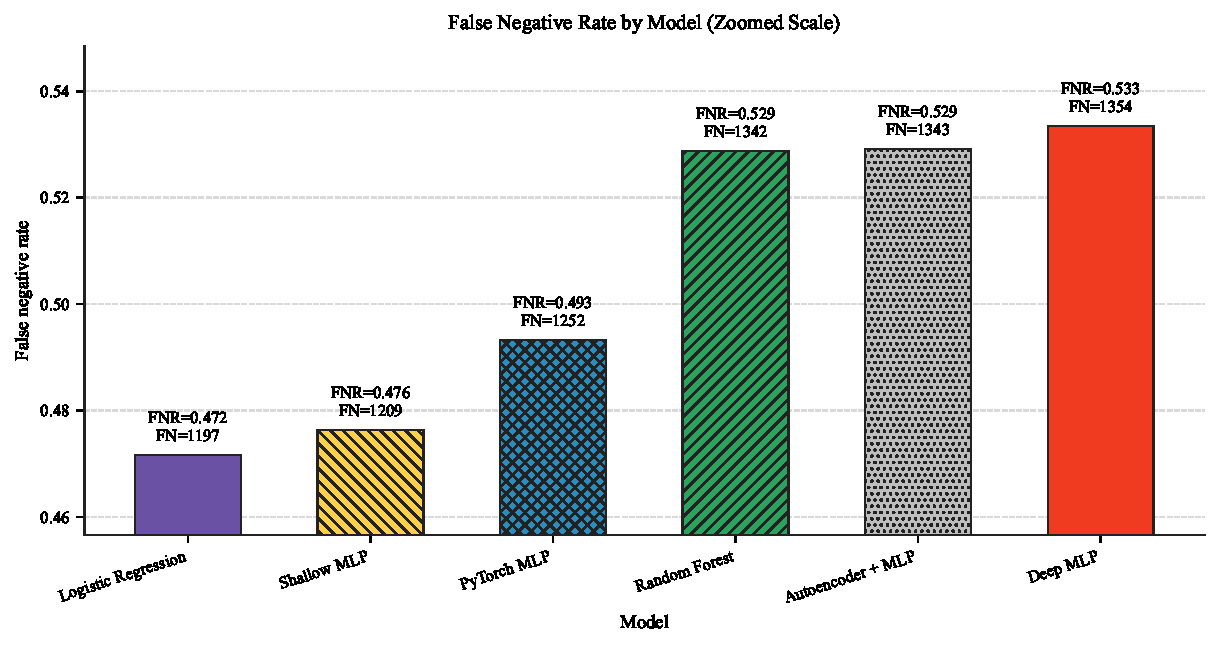
\includegraphics[width=\linewidth]{reports/final_run/false_negative_rate.pdf}
  \caption{Zoomed y-axis로 표시한 모델별 false-negative rate. IDS security coverage에서는 낮을수록 좋다.}
  \Description{여섯 개 평가 모델의 false-negative rate와 false-negative count를 비교하는 zoomed bar chart.}
  \label{fig:fnr}
\end{figure}

\begin{figure*}[t]
  \centering
  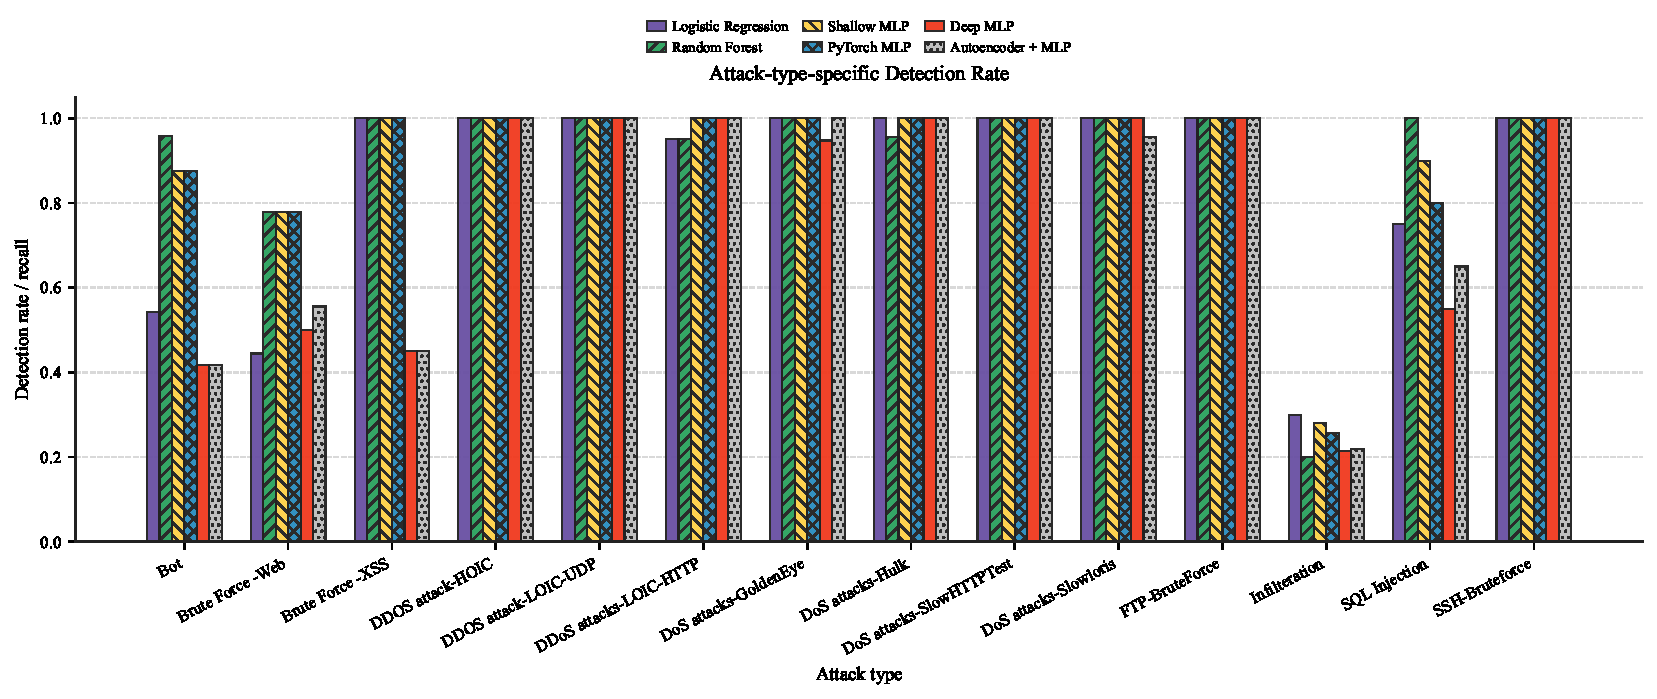
\includegraphics[width=\textwidth]{reports/final_run/attack_type_detection.pdf}
  \caption{Fine-grained attack type별 model recall.}
  \Description{각 모델의 fine-grained attack-type recall을 보여주는 grouped bar chart.}
  \label{fig:types}
\end{figure*}

\subsection{Coarse Attack-Family Results}

Table~\ref{tab:families}는 coarse attack family별 가장 강한 모델을 요약한다.
Family-level result는 aggregate metric에 attack-type context가 필요한 이유를 보여준다.
IDS task의 난이도는 attack family에 강하게 의존한다.
DoS/DDoS는 tested model들에서 거의 해결된 category였다.
Shallow MLP와 PyTorch MLP는 DoS/DDoS family에서 1.000 recall을 달성했다.
Random Forest는 Botnet과 Web Attack에서 가장 강했다.
Brute Force에서는 Random Forest, Shallow MLP, PyTorch MLP가 0.932 recall로 동률이었다.

가장 중요한 결과는 Infiltration family이다.
Infiltration은 1,669개 test attack을 포함했지만, 가장 좋은 Logistic Regression도 499개만 탐지했다.
Family-level recall은 0.299에 불과했다.
Random Forest는 334개, Shallow MLP는 469개, PyTorch MLP는 428개, Deep MLP는 359개, Autoencoder + MLP는 367개를 탐지했다.
이 family는 전체 false negative의 큰 부분을 차지한다.

\begin{table}[t]
  \caption{Coarse attack-family recall 기준 best model.}
  \label{tab:families}
  \centering
  \small
  \begin{tabular}{lll}
    \toprule
    Family & Best model & Recall \\
    \midrule
    Botnet & Random Forest & 0.958 \\
    Brute Force & RF / Shallow MLP / PyTorch MLP & 0.932 \\
    DoS/DDoS & Shallow MLP / PyTorch MLP & 1.000 \\
    Infiltration & Logistic Regression & 0.299 \\
    Web Attack & Random Forest & 1.000 \\
    \bottomrule
  \end{tabular}
\end{table}

\subsection{Fine-Grained Attack-Type Results}

이 subsection은 본 논문의 핵심 결과를 가장 직접적으로 보여준다.
앞의 aggregate metric과 family-level result가 전체적인 경향을 보여준다면, fine-grained attack-type result는 어떤 구체적 attack이 실제로 covered되거나 uncovered로 남는지를 보여준다.
따라서 이 분석은 단순히 추가적인 세부 결과가 아니라, aggregate IDS metric이 숨길 수 있는 security-relevant blind spot을 확인하는 중심 evidence이다.
Fine-grained result는 family-level pattern을 만드는 구체적인 attack을 설명한다.
또한 aggregate model score가 하나의 숫자로 압축해버리는 구체적인 failure mode를 보여준다.
여기서 attack-type-specific evaluation은 post-hoc explanation을 넘어 practical model selection의 근거가 된다.
이 분석은 어떤 모델이 전체적으로 좋아 보이는지만이 아니라, 각 모델이 어떤 attack label을 실제로 cover하는지 보여주기 때문이다.
몇몇 attack label은 거의 모든 모델이 완벽하게 탐지했다.
DDOS attack-HOIC, DDOS attack-LOIC-UDP, DoS attacks-SlowHTTPTest, FTP-BruteForce, SSH-Bruteforce는 대부분 모델에서 near-perfect 또는 perfect recall을 보였다.
이 attack들은 benign traffic과 구분되는 flow-feature signature가 비교적 뚜렷한 것으로 보인다.

Table~\ref{tab:finegrained}는 이 분석에 사용된 per-label recall을 보여준다.
이 표는 best model이 attack type에 따라 달라진다는 점을 보여준다.
또한 dataset 전체의 난이도가 균등하지 않다는 점도 보여준다.
일부 row는 거의 해결되었지만, Infilteration은 여섯 모델 모두에서 일관되게 약했다.

\begin{table}[t]
  \caption{Fine-grained attack-type recall by model. LR = Logistic Regression, RF = Random Forest, Shallow = Shallow MLP, PT = PyTorch MLP, Deep = Deep MLP, AE = Autoencoder + MLP.}
  \label{tab:finegrained}
  \centering
  \scriptsize
  \setlength{\tabcolsep}{2pt}
  \resizebox{\columnwidth}{!}{%
  \begin{tabular}{lrrrrrrr}
    \toprule
    Attack type & Test & LR & RF & Shallow & PT & Deep & AE \\
    \midrule
    Bot & 24 & 0.542 & 0.958 & 0.875 & 0.875 & 0.417 & 0.417 \\
    Brute Force -Web & 18 & 0.444 & 0.778 & 0.778 & 0.778 & 0.500 & 0.556 \\
    Brute Force -XSS & 20 & 1.000 & 1.000 & 1.000 & 1.000 & 0.450 & 0.450 \\
    DDOS attack-HOIC & 618 & 1.000 & 1.000 & 1.000 & 1.000 & 1.000 & 1.000 \\
    DDOS attack-LOIC-UDP & 15 & 1.000 & 1.000 & 1.000 & 1.000 & 1.000 & 1.000 \\
    DDoS attacks-LOIC-HTTP & 20 & 0.950 & 0.950 & 1.000 & 1.000 & 1.000 & 1.000 \\
    DoS attacks-GoldenEye & 19 & 1.000 & 1.000 & 1.000 & 1.000 & 0.947 & 1.000 \\
    DoS attacks-Hulk & 23 & 1.000 & 0.957 & 1.000 & 1.000 & 1.000 & 1.000 \\
    DoS attacks-SlowHTTPTest & 28 & 1.000 & 1.000 & 1.000 & 1.000 & 1.000 & 1.000 \\
    DoS attacks-Slowloris & 23 & 1.000 & 1.000 & 1.000 & 1.000 & 1.000 & 0.957 \\
    FTP-BruteForce & 18 & 1.000 & 1.000 & 1.000 & 1.000 & 1.000 & 1.000 \\
    Infilteration & 1669 & 0.299 & 0.200 & 0.281 & 0.256 & 0.215 & 0.220 \\
    SQL Injection & 20 & 0.750 & 1.000 & 0.900 & 0.800 & 0.550 & 0.650 \\
    SSH-Bruteforce & 23 & 1.000 & 1.000 & 1.000 & 1.000 & 1.000 & 1.000 \\
    \bottomrule
  \end{tabular}
  }
\end{table}

\paragraph{DDoS attacks-LOIC-HTTP.}
DDoS attacks-LOIC-HTTP는 neural model이 조금 더 안정적으로 보인 case이다.
Shallow MLP, PyTorch MLP, Deep MLP, Autoencoder + MLP는 모두 1.000 recall을 달성했고, Logistic Regression과 Random Forest는 각각 1개 sample을 놓쳤다.
이는 제한적인 의미에서 hypothesis를 지지한다.
일부 attack type에서는 neural model이 traditional baseline을 match하거나 약간 개선했다.

\paragraph{Bot.}
Bot traffic은 반대 pattern을 보였다.
Random Forest는 0.958 recall을 달성했지만, Logistic Regression은 0.542였고 deep neural model은 낮았다.
Deep MLP와 Autoencoder + MLP는 각각 Bot에서 0.417 recall에 그쳤다.
이는 이 small category에서 tree-based model이 유용한 feature threshold를 더 잘 포착했을 가능성을 보여준다.

\paragraph{Brute Force -Web.}
Brute Force -Web은 feature interaction을 표현할 수 있는 모델에 유리했다.
Random Forest, Shallow MLP, PyTorch MLP는 모두 0.778 recall을 달성했지만, Logistic Regression은 0.444에 그쳤다.
\paragraph{Brute Force -XSS.}
Brute Force -XSS는 deeper neural model이 rare label에서 항상 더 robust하지 않다는 점을 보여준다.
Logistic Regression, Random Forest, Shallow MLP, PyTorch MLP는 1.000 recall을 달성했지만, Deep MLP와 Autoencoder + MLP는 0.450에 그쳤다.

\paragraph{SQL Injection.}
SQL Injection은 Random Forest가 1.000 recall로 가장 강했다.
Shallow MLP도 0.900으로 양호했지만, Logistic Regression은 0.750, PyTorch MLP는 0.800, Deep MLP는 0.550, Autoencoder + MLP는 0.650이었다.
이는 web-related attack에서 Random Forest가 여전히 경쟁력 있고 때로는 우수하다는 broader result를 지지한다.

\paragraph{Infilteration.}
가장 중요한 fine-grained attack label은 Infilteration이다.
Test set에서 가장 큰 attack label이며 1,669개 sample을 포함한다.
모든 모델이 이 label에서 낮은 성능을 보였다.
Logistic Regression이 0.299 recall로 가장 좋았고, Shallow MLP는 0.281, PyTorch MLP는 0.256, Autoencoder + MLP는 0.220, Deep MLP는 0.215, Random Forest는 0.200이었다.
이것이 실험에서 가장 명확한 security blind spot이다.

\section{Discussion}

종합하면, 이 결과는 attack-type-specific evaluation의 역할을 단순한 post-hoc explanation에서 practical model selection으로 확장한다.
Precision, recall, F1-score 같은 aggregate metric은 평균적으로 좋은 모델을 빠르게 비교하는 데 유용하지만, 그 모델이 특정 IDS 환경에서 중요한 attack family를 실제로 cover하는지는 보여주지 못한다.
이번 실험에서도 neural model은 일부 aggregate metric을 개선했지만, 그것이 곧 더 넓은 security coverage를 의미하지는 않았다.
따라서 IDS evaluation의 핵심은 “어떤 모델이 전체 점수에서 이겼는가”가 아니라, “그 모델이 이긴 뒤에도 어떤 attack을 놓치는가”여야 한다.
Attack-type-specific analysis는 이 질문에 답하기 위한 필수적인 평가 단계이며, future IDS model selection과 hybrid design을 더 유연하게 만드는 근거가 된다.

\paragraph{Metric choice.}
이 결과의 핵심은 평가 기준에 따라 결론이 달라진다는 점이다.
F1-score나 precision만 보면 Deep MLP가 가장 좋은 모델처럼 보인다.
하지만 IDS에서는 “탐지한 alert가 얼마나 정확한가”만큼 “공격을 얼마나 놓치지 않는가”도 중요하다.
이 기준으로 보면 Logistic Regression과 Shallow MLP가 더 안전한 선택으로 보인다.
따라서 neural model은 일부 attack family와 aggregate score를 개선했지만, missed attack을 일관되게 줄이지는 못했다.

\paragraph{Attack-type blind spots.}
Attack-type result는 이 mismatch가 생기는 이유를 보여준다.
DoS/DDoS와 FTP/SSH brute-force traffic은 대부분 잘 탐지되었고, Bot과 SQL Injection에서는 Random Forest가 특히 강했다.
반면 Infiltration은 frequent하면서도 어려운 shared blind spot이었다.
모든 모델이 Infiltration sample의 대부분을 놓쳤고, 여섯 모델에서 Infiltration은 전체 false negative의 96.8\%에서 99.5\%를 차지했다.
따라서 attack-type-specific evaluation은 단순한 보조 설명이 아니라 diagnostic tool이다.
모델별 강점은 어떤 traffic pattern을 잘 탐지하는지 보여주고, 공통 실패는 feature, dataset, 또는 binary objective의 한계를 시사한다.

\paragraph{Operational choice.}
운영 관점에서 best model은 평균 점수가 아니라 어떤 attack을 반드시 잡아야 하는지에 따라 선택되어야 한다.
False alarm을 줄이는 것이 중요하다면 Deep MLP나 Autoencoder + MLP가 매력적일 수 있지만, missed attack을 줄이는 것이 더 중요하다면 Logistic Regression이나 Shallow MLP가 더 나은 선택일 수 있다.
같은 논리는 future hybrid IDS 설계에도 연결된다.
모든 malicious traffic에 하나의 global decision rule을 적용하기보다, attack family별 threshold를 다르게 두거나 여러 모델의 signal을 조합할 수 있다.
Autoencoder + MLP 결과도 이 점을 강화한다.
Representation learning은 selectivity를 높였지만 false-negative problem을 해결하지 못했으므로, 더 깊거나 복잡한 모델이 자동으로 security coverage를 높인다고 가정해서는 안 된다.

\section{Risks and Limitations}

첫 번째 limitation은 dataset dependence이다.
CSE-CIC-IDS2018은 public benchmark dataset이며, 모델이 general intrusion behavior가 아니라 dataset-specific artifact를 학습했을 수 있다.
이 위험을 줄이기 위해 본 연구는 accuracy-only reporting을 피하고 attack type별 false negative에 집중했다.
하지만 결과는 여전히 production IDS guarantee가 아니라 sampled benchmark에서 관찰된 behavior로 해석해야 한다.

두 번째 limitation은 class imbalance이다.
일부 attack type은 test support가 작기 때문에 perfect recall을 과도하게 해석하면 안 된다.
예를 들어 몇몇 rare attack category는 test sample이 30개 미만이다.
따라서 분석은 frequent하면서도 poorly detected된 Infiltration에 특별히 주목했다.

세 번째 limitation은 model tuning이다.
Neural model은 exhaustively tuned architecture가 아니라 reproducible baseline으로 구현되었다.
다른 threshold, loss function, resampling strategy, hyperparameter가 recall을 개선할 수 있다.
특히 default 0.5 decision threshold는 security objective에 최적이 아닐 수 있다.

네 번째 limitation은 binary training objective이다.
모델은 benign과 malicious flow를 구분하도록 학습되었고, attack label은 training 이후 analysis에만 사용되었다.
Multiclass 또는 hierarchical model은 attack-specific pattern을 더 직접적으로 학습할 수 있다.
Binary design은 lightweight IDS prototype에 맞고 비교를 단순하게 유지하기 위해 선택했다.

\section{Future Work}

첫 번째 next step은 security objective에 맞춘 threshold tuning이다.
고정된 0.5 threshold 대신 false positive를 통제하면서 false negative를 줄이는 threshold를 각 모델별로 찾아야 한다.
이것은 Deep MLP와 Autoencoder + MLP가 precision 일부를 포기하고 recall을 개선할 수 있는지 직접 테스트한다.
Precision-recall curve나 fixed false-positive budget에서의 recall을 함께 보고하면 alert volume이 제한된 operational IDS 상황에 더 가까운 비교가 가능하다.

두 번째 next step은 Infiltration에 대한 targeted improvement이다.
Infiltration이 missed attack의 대부분을 차지하므로, 이 category의 feature distribution을 inspect하고 benign flow와 비교하며 resampling 또는 cost-sensitive training이 detection을 개선하는지 확인해야 한다.
이 작업은 main security blind spot을 직접 다루기 때문에 단순히 모델 종류를 더 늘리는 것보다 우선순위가 높다.
목표는 Infiltration이 어려운 이유가 class imbalance, benign flow와의 feature overlap, sampling artifact, 또는 binary training objective 때문인지 구분하는 것이다.

세 번째 next step은 multiclass 또는 hierarchical classification이다.
모델이 먼저 malicious traffic을 탐지한 뒤 attack family를 분류할 수 있다.
또는 attack-family label을 training에 사용해 category-specific feature를 학습하도록 만들 수 있다.
이 방식은 모든 malicious flow를 하나의 positive class로 합쳤을 때 보이지 않던 pattern이 attack supervision을 통해 학습되는지 확인할 수 있다.
또 다른 방향은 hybrid ensemble이다.
예를 들어 web 및 botnet-like traffic에는 Random Forest signal을 더 크게 반영하고, high-volume DoS/DDoS 또는 brute-force traffic에는 MLP-style model을 더 크게 반영할 수 있다.

네 번째 next step은 broader validation이다.
현재 연구는 CSE-CIC-IDS2018을 사용했다.
같은 pipeline을 CICIDS2017 또는 다른 flow-level IDS dataset에 적용하면 attack-specific conclusion이 하나의 benchmark를 넘어 generalize되는지 확인할 수 있다.
같은 model ranking과 blind spot이 여러 dataset에서 반복된다면 결론은 더 강해지고, 달라진다면 IDS model selection이 dataset-dependent하다는 점을 보여준다.

\section{Conclusion}

\paragraph{Attack-type-specific evaluation.}
가장 강한 결론은 IDS evaluation이 attack-type-specific이어야 한다는 점이다.
이 논문은 flow-level intrusion detection에서 aggregate metric만으로는 IDS의 보안 성능을 충분히 설명할 수 없다는 점을 보였다.
Precision, recall, F1-score는 모델을 한눈에 비교하는 데 유용하지만, 그 숫자만으로는 어떤 attack type이 여전히 탐지되지 않는지 알기 어렵다.
따라서 IDS evaluation의 중심 질문은 “어떤 모델이 전체 점수에서 가장 높았는가”가 아니라, “그 모델이 어떤 attack type을 여전히 uncovered로 남기는가”여야 한다. 이번 CSE-CIC-IDS2018 experiment는 이 결론을 구체적으로 보여준다.
일부 모델은 aggregate F1-score나 precision에서 더 좋아 보였지만, attack-type별로 보면 다른 그림이 나타났다.
DoS/DDoS와 여러 brute-force attack은 대부분 잘 탐지되었지만, Infiltration은 모든 모델에서 공통적인 blind spot으로 남았다.
가장 좋은 Infiltration recall도 0.299에 그쳤고, Infiltration은 모델별 false negative의 96.8\%에서 99.5\%를 차지했다.
이 결과는 전체 평균 점수가 좋아 보여도, 실제 missed attack은 특정 attack type에 집중될 수 있음을 보여준다. 따라서 attack-type-specific analysis는 부가적인 해석 단계가 아니라 IDS evaluation의 핵심 단계가 되어야 한다.
모델이 secure한지는 평균 점수가 높기 때문이 아니라, 중요한 attack type을 얼마나 적게 놓치는지에 따라 판단되어야 한다.
Attack-type-specific evaluation은 aggregate metric이 숨기는 blind spot을 드러내고, 모델의 실제 security coverage를 더 정확히 보여준다.

\paragraph{Flexible model choice.}
동시에 이 분석은 IDS model 선택의 유연성도 제공한다.
Attack-type-specific result를 보면 하나의 모델이 모든 attack type에서 일관되게 우수한 것은 아니었다.
어떤 모델은 Bot이나 SQL Injection처럼 특정 attack type에서 더 강했고, 다른 모델은 brute-force 또는 DoS/DDoS traffic에서 더 안정적으로 작동했다.
따라서 attack-type-specific evaluation은 단순히 약점을 찾는 방법이 아니라, 어떤 보안 목표에 어떤 모델이 더 적합한지 판단하는 기준이 된다. 이 점은 IDS design을 더 유연하게 만든다.
만약 운영 환경에서 Botnet이나 Web Attack coverage가 더 중요하다면, Random Forest처럼 해당 attack type에서 강한 모델을 우선 고려할 수 있다.
반대로 missed attack을 전체적으로 줄이는 것이 더 중요하다면, recall이 높은 모델을 선택하는 것이 더 적절할 수 있다.
즉 attack-type-specific evaluation은 하나의 global winner를 고르는 대신, threat priority에 따라 model choice를 조정할 수 있게 한다. 또한 이 분석은 여러 모델을 조합하는 근거도 제공한다.
각 모델이 서로 다른 attack type에 강하다면, future IDS는 하나의 모델에만 의존하지 않고 model signal을 조합하거나 attack-family별 threshold를 다르게 설정할 수 있다.
이런 접근은 aggregate score만 보고 모델을 선택하는 방식보다 더 현실적인 security coverage를 제공할 수 있다.
따라서 이 논문의 핵심 함의는 IDS evaluation이 model-level leaderboard에만 머물러서는 충분하지 않다는 점이다.
Aggregate score와 함께 attack-type-level coverage를 평가할 때, 모델의 실제 security coverage를 더 현실적으로 이해할 수 있다.

\clearpage

\begin{thebibliography}{6}

\bibitem{gamage2020}
S. Gamage and J. Samarabandu. 2020. Deep Learning Methods in Network Intrusion Detection: A Survey and an Objective Comparison. Journal of Network and
Computer Applications 169, 102767.

\bibitem{saito2015}
T. Saito and M. Rehmsmeier. 2015. The Precision-Recall Plot Is More Informative
than the ROC Plot When Evaluating Binary Classifiers on Imbalanced Datasets.
PLOS ONE 10, 3, e0118432. https://doi.org/10.1371/journal.pone.0118432

\bibitem{cic2018}
Canadian Institute for Cybersecurity. 2018. CSE-CIC-IDS2018 on AWS: A Realistic
Cyber Defense Dataset. University of New Brunswick. https://www.unb.ca/cic/
datasets/ids-2018.html

\bibitem{breiman2001}
L. Breiman. 2001. Random Forests. Machine Learning 45, 1, 5--32. https://doi.org/
10.1023/A:1010933404324

\bibitem{rosay2020}
A. Rosay, F. Carlier, and P. Leroux. 2020. MLP4NIDS: An Efficient MLP-Based
Network Intrusion Detection for CICIDS2017 Dataset. In Machine Learning for
Networking (MLN 2019), Lecture Notes in Computer Science 12081, 240--254.
https://doi.org/10.1007/978-3-030-45778-5\_16

\bibitem{song2021}
Y. Song, S. Hyun, and Y.-G. Cheong. 2021. Analysis of Autoencoders for Network
Intrusion Detection. Sensors 21, 13, 4294. https://doi.org/10.3390/s21134294

\end{thebibliography}

\end{document}
